%% ---------------------------------------------------------------------------
%% paper_analog_probabilistic.tex
%% Probabilistic Analog Forecasting of Day-Ahead Locational Marginal Prices
%% Uriel Iram Lezama-Lope
%%
%% Format: Journal of Forecasting (Wiley).
%% Single column, one-and-a-half spacing, line numbers for review, APA
%% citations and references via apacite, at most six keywords, single-blind
%% review (author details are kept in the manuscript).
%% Compile with: pdflatex -> bibtex -> pdflatex -> pdflatex
%%
%% For the accepted version Wiley asks for its own class (wileyNJD-v2),
%% available in Overleaf as the "Wiley NJD" template: only the preamble
%% changes, the body below is unaffected.
%% ---------------------------------------------------------------------------

\documentclass[12pt,a4paper]{article}

\usepackage[utf8]{inputenc}
\usepackage[T1]{fontenc}
\usepackage[english]{babel}
\usepackage{amsmath,amssymb}
\usepackage{graphicx}
\usepackage{booktabs}
\usepackage{url}
\usepackage[margin=2.5cm]{geometry}
\usepackage{setspace}
\usepackage[natbibapa]{apacite}
\usepackage[hidelinks]{hyperref}
\usepackage{lineno}
\usepackage{caption}
\captionsetup{font=small,labelfont=bf}

%% lineno y amsmath chocan en los entornos de ecuación: este parche, estándar,
%% los reconcilia para que las ecuaciones queden numeradas y con su renglón.
\newcommand*\patchAmsMathEnvironmentForLineno[1]{%
  \expandafter\let\csname old#1\expandafter\endcsname\csname #1\endcsname
  \expandafter\let\csname oldend#1\expandafter\endcsname\csname end#1\endcsname
  \renewenvironment{#1}%
    {\linenomath\csname old#1\endcsname}%
    {\csname oldend#1\endcsname\endlinenomath}}%
\newcommand*\patchBothAmsMathEnvironmentsForLineno[1]{%
  \patchAmsMathEnvironmentForLineno{#1}%
  \patchAmsMathEnvironmentForLineno{#1*}}%
\AtBeginDocument{%
  \patchBothAmsMathEnvironmentsForLineno{equation}%
  \patchBothAmsMathEnvironmentsForLineno{align}%
  \patchBothAmsMathEnvironmentsForLineno{gather}%
  \patchBothAmsMathEnvironmentsForLineno{multline}%
}

\renewcommand{\arraystretch}{1.15}
\onehalfspacing
\linenumbers

\title{\bfseries Probabilistic Analog Forecasting of Day-Ahead Locational
Marginal Prices: An Ensemble of Pairwise Analog Regressions}

\author{Uriel Iram Lezama-Lope$^{a}$ \quad
Adriana Gonz\'alez-Urquiza$^{b}$ \quad
Guillermo Santamar\'ia-Bonfil$^{c}$ \\[0.7em]
\normalsize $^{a}$ Independent Researcher, Mexico.
ORCID: 0000-0002-3541-7194.
\texttt{ilezama.ceme@gmail.com} \\
\normalsize $^{b}$ CFE Internacional, Mexico. \\
\normalsize $^{c}$ BBVA Mexico, Data Portfolio Manager Department, Unique
Experience and Data General Directorate, Mexico. \\
\normalsize \phantom{$^{c}$} ORCID: 0000-0003-4302-4902.
\texttt{guillermo.santamaria@bbva.com} \\[0.4em]
\normalsize Corresponding author: Uriel Iram Lezama-Lope.}

\date{\today}

\newcommand{\NORIGINS}{92}
\newcommand{\NFORECASTS}{2208}
\newcommand{\TESTSTART}{2026-03-01}
\newcommand{\TESTEND}{2026-08-31}
\newcommand{\KANALOGS}{40}
\newcommand{\VSELE}{48}
\newcommand{\HORIZON}{24}
\newcommand{\APCRPS}{62.3}
\newcommand{\APREL}{0.216}
\newcommand{\APTIME}{0.027}
\newcommand{\APCOVNINETYFIVE}{77.8}
\newcommand{\APCOVEIGHTY}{66.8}
\newcommand{\APWINK}{1\,139}
\newcommand{\APMAE}{156.2}
\newcommand{\APPINNINETYFIVE}{39.33}
\newcommand{\APSHARPNINETYFIVE}{515}
\newcommand{\SNREL}{0.181}
\newcommand{\SNSHARPNINETYFIVE}{848}
\newcommand{\SNCOVNINETYFIVE}{90.4}
\newcommand{\LGBMCOVNINETYFIVE}{68.6}
\newcommand{\LGBMTIME}{0.044}
\newcommand{\ARIMATIME}{65.7}
\newcommand{\SPEEDUP}{2\,417}
\newcommand{\CRPSGAINARIMA}{22.2}
\newcommand{\CRPSGAINLGBM}{8.3}
\newcommand{\CRPSGAINRAW}{21.1}
\newcommand{\CLIPRATE}{0.32}
\newcommand{\NCAL}{72}
\newcommand{\CALCOV}{89.4}
\newcommand{\CALCOVRAW}{77.8}
\newcommand{\CALCRPS}{69.7}
\newcommand{\CALCRPSRAW}{70.2}
\newcommand{\CALSHARP}{1\,059}
\newcommand{\CALSHARPRAW}{565}
\newcommand{\CALWINK}{1\,435}
\newcommand{\CALWINKRAW}{1\,271}
\newcommand{\NSENS}{30}
\newcommand{\SENSBESTV}{168}
\newcommand{\SENSBESTK}{20}
\newcommand{\SENSBESTTOL}{0.5}
\newcommand{\SENSBESTCRPS}{50.7}
\newcommand{\SENSTMIN}{0.003}
\newcommand{\SENSTMAX}{0.248}
\newcommand{\ABANENCRPS}{79.0}
\newcommand{\ABANENCOV}{81.5}
\newcommand{\ABANENREL}{0.257}
\newcommand{\ABANENSHARP}{806}
\newcommand{\ABANENPIN}{62.80}
\newcommand{\ABDUDCRPS}{61.0}
\newcommand{\ABDUDCOV}{84.1}
\newcommand{\ABDUDREL}{0.197}
\newcommand{\ABDUDSHARP}{619}
\newcommand{\ABDUDPIN}{37.22}
\newcommand{\ABOLSCRPS}{62.3}
\newcommand{\ABOLSCOV}{77.8}
\newcommand{\ABOLSREL}{0.216}
\newcommand{\ABOLSSHARP}{515}
\newcommand{\ABOLSPIN}{39.33}
\newcommand{\ABNOCLIPCRPS}{62.5}
\newcommand{\ABNOCLIPCOV}{77.8}
\newcommand{\ABNOCLIPREL}{0.216}
\newcommand{\ABNOCLIPSHARP}{534}
\newcommand{\ABNOCLIPPIN}{40.24}
\newcommand{\ABOLSGAINANEN}{21.1}
\newcommand{\SENSAPRIORI}{52.8}
\newcommand{\SENSGAP}{3.9}


\begin{document}

\maketitle

\noindent\textbf{Running title:} Probabilistic analog price forecasts

\section*{Acknowledgements}
The authors thank the National Center of Energy Control (CENACE), the
institution in charge of the operational control of the Mexican wholesale
electricity market, for publishing the price data used in this work. This
research received no specific grant from any funding agency in the public,
commercial or not-for-profit sectors.

\section*{Statements}

\noindent\textbf{Data availability statement.} The day-ahead locational
marginal prices analysed in this study are published by the National Center of
Energy Control (CENACE) of Mexico and are openly available from its public
information system. The backtest code, the evaluation scripts and the
aggregated results that generate every table and figure in this paper are
available from the corresponding author upon reasonable request.

\noindent\textbf{Funding statement.} This research received no specific grant
from any funding agency in the public, commercial or not-for-profit sectors.

\noindent\textbf{Conflict of interest disclosure.} The authors declare no
conflict of interest.

\noindent\textbf{Disclaimer.} The third author wishes to clarify that the
present work represents his own opinion and research lines, and not
necessarily the opinion of BBVA Mexico.

\noindent\textbf{Ethics approval statement.} This study did not involve human
participants or animals, and therefore required no ethics approval.

\noindent\textbf{Permission to reproduce material from other sources.} No
material from other sources is reproduced in this article.

\bigskip

\begin{abstract}
\noindent
The analog method forecasts a time series by searching the past for stretches
that resemble the present one, fitting a regression between each of them and
the present, and carrying that relation forward. In its point form it is
already known to be fast and accurate for very short-term forecasting. This
paper makes its analog stage probabilistic: instead of pooling the retrieved
analogs into one regression that returns a single number per hour, one
regression is fitted per analog and propagated separately, so that every
analog contributes a complete future trajectory and the empirical quantiles of
the resulting ensemble are the forecast. The method is tested on day-ahead
hourly electricity prices of a node of the Mexican wholesale market against a
seasonal benchmark, an exponential smoothing method, an automatically selected
autoregressive model and a quantile gradient boosting. Against all four of them it attains the best
score of every kind measured here, including the loss on the expensive side of
the distribution that a buyer actually pays, and it does so in a few
hundredths of a second, some two thousand times faster than the autoregressive
model; every difference is statistically significant. Its intervals are nevertheless too narrow: the
nominal ninety-five per cent interval covers seventy-eight per cent of the
observations. A recalibration that uses only the errors of past forecast
origins restores most of the missing coverage without improving the score. Two
ablations show that the gain over a plain analog ensemble comes from rescaling
each analog to the level of the present, not from the search itself, and that
shrinking that rescaling, as least squares does, costs coverage without buying
accuracy.
\end{abstract}

\noindent\textbf{Keywords:} probabilistic forecasting; analog ensemble;
electricity price forecasting; prediction intervals; reliability; energy
markets

\vspace{1em}

\section{Introduction}

Short-term forecasts of electricity prices and load are used to take decisions
that have a price: how much energy to buy in the day-ahead market, how much
exposure to leave for real time, how much to hedge. A single number per hour
does not carry the information those decisions need. What a buyer needs to
know is not only where the price is expected to land but how far it can go on
the expensive side, because the cost of being wrong is not symmetric: a peak
that was not anticipated is paid at the real-time price, while a slightly
conservative purchase costs almost nothing. That asymmetry is the practical
reason to move from point forecasts to forecasts that state a whole
distribution \citep{Hong2016,Nowotarski2018}.

Two lines of our own work meet in this paper. The first is the analog method
with moving-average correction (AnMA), reported by \citet{LezamaLope2023} for
very short-term load forecasting: it searches the history for the stretches
most similar to the most recent data, regresses the present on those analogs,
and applies the fitted relation to what followed each analog in the past. The
method is accurate, it has no training stage, and it is orders of magnitude
cheaper than the machine-learning alternatives it was compared against. The
second is an earlier, unpublished comparison of three probabilistic load
forecasting schemes built on similar days, prepared by the present authors
with colleagues at the National Institute of Electricity and Clean Energies
(INEEL), in which the spread of several regressions on similar days was turned
into quantiles and evaluated with reliability and sharpness. That work kept the ensemble implicit: the
regressions were built one per similar day, over a window of a few months, for
a horizon of ten periods, on aggregated regional load.

Here we take the second idea seriously and make it the method. What we make
probabilistic is the analog stage; the moving-average correction that
completes AnMA acts on residuals and is left out, so the comparison below is
between the analog stage and the benchmarks, not between AnMA and the
benchmarks. The change is
small to state and large in consequence. In its point form, the analog method
pools the $k$ analogs as $k$ columns of one design matrix and returns one
fitted value per step. In the probabilistic form we propose, each analog is
regressed against the present on its own, and each fitted relation is
propagated through the future of that analog. The result is not one path but
$k$ paths, each of which answers a well-posed question: \emph{if the relation
that held between this past episode and the present were to hold forward, what
would happen?} The ensemble of those $k$ answers is a non-parametric
predictive distribution, obtained without distributional assumptions, without
a training phase and without a residual model.

The contribution of this paper is fourfold. First, we give the formulation of
the probabilistic analog method and place it in a family that also contains
the analog ensembles used in meteorology
\citep{DelleMonache2013,Alessandrini2015} and the pattern rescaling of
local-regression models \citep{Dudek2016}, which differ from it only in one
coefficient; we also separate it from quantile regression averaging on sister
forecasts \citep{Liu2017}, with which it is easily confused. Second, we
evaluate it on a problem that is harder than aggregated load: the hourly
day-ahead locational marginal price of a single node, a series with spikes,
regime changes and heavy upper tails. Third, we report a like-for-like
comparison against four probabilistic benchmarks on the same origins, with the
same scores and with significance tests, including computing time, which is the
constraint that decides whether a method can be run every day for hundreds of
nodes. Fourth, we show where the construction fails — its intervals are
narrower than they should be — measure that failure, and report what a simple
recalibration does and does not fix.

The rest of the paper is organized as follows. Section~\ref{sec:methods}
describes the data, the method, the benchmarks and the evaluation. Section
\ref{sec:results} reports the backtest. Section~\ref{sec:discussion} discusses
what the numbers do and do not support, and Section~\ref{sec:conclusions}
concludes.

\section{Materials and Methods}
\label{sec:methods}

\subsection{Data}
\label{sec:data}

We use the hourly day-ahead locational marginal price (LMP) of the San Juan
del R\'io node of the Mexican wholesale electricity market, published by the
national energy control centre (CENACE) and kept in a local database
maintained for this and related work. The series runs from 4 April 2018 to 23 September 2026 and has
74,276 hourly observations; four missing hours, caused by publication
gaps, were filled by linear interpolation. Prices are in Mexican pesos per
megawatt-hour (MXN/MWh).

The series is a demanding target. Over the sample its mean is about
959 MXN/MWh and its median about 751 MXN/MWh, but its maximum
exceeds 26,000 MXN/MWh and it takes negative values in a small number of
hours. The distance between mean and median, together with the size of the
extremes, is exactly what makes a point forecast insufficient and a
well-calibrated upper tail valuable.

\subsection{The analog method in point form}
\label{sec:analog}

Let $S=(s_1,\dots,s_p)$ be the observed series up to the present. The present
window is the last $v_1$ observations,
\begin{equation}
Y=(s_{p-v_1+1},\dots,s_p),
\end{equation}
where $v_1$ is chosen longer than the forecast horizon $v_2$. Every
sub-sequence of length $v_1$ that ends at least $v_2$ periods before the
present is a candidate analog. For each candidate $X_i=(s_i,\dots,s_{i+v_1-1})$
we measure similarity to the present with the Pearson correlation
coefficient,
\begin{equation}
\rho_i \;=\; \frac{\sum_{j=1}^{v_1}\big(x_{i+j-1}-\bar{X_i}\big)
\big(y_j-\bar{Y}\big)}{\sigma_{X_i}\,\sigma_{Y}},
\end{equation}
and keep the $k$ candidates with the highest $\rho_i$, subject to a separation
rule: a candidate starting at position $i$ is rejected if an already accepted
analog starts at a position $j$ with $|i-j| < \delta v_1$, with
$\delta\in(0,1]$. The rule prevents the ensemble from being filled with
shifted copies of the same episode \citep{LezamaLope2023}.

Write $X_{(1)},\dots,X_{(k)}$ for the accepted analogs and
$X'_{(1)},\dots,X'_{(k)}$ for what followed each of them, that is, the $v_2$
observations immediately after each analog window. In the point version of the
method, the $k$ analogs are the regressors of a single least-squares model of
the present,
\begin{equation}
Y \;=\; \beta_0 + \sum_{i=1}^{k}\beta_i X_{(i)} + \varepsilon ,
\end{equation}
and the forecast is $\hat{Y}' = \hat\beta_0 + \sum_i \hat\beta_i X'_{(i)}$: one
trajectory, one number per step.

\subsection{The probabilistic analog method}
\label{sec:prob}

The proposed method replaces the single $k$-regressor model by $k$ pairwise
models. For each analog $i$ we fit, by ordinary least squares on the $v_1$
pairs $(x_{i,j},y_j)$ matched by position inside the window,
\begin{equation}
\bigl(\hat a_i,\hat b_i\bigr)=\arg\min_{a,b}
\sum_{j=1}^{v_1}\bigl(y_j-a-b\,x_{i,j}\bigr)^2 ,
\qquad
\hat b_i=\rho_i\frac{\sigma_Y}{\sigma_{X_i}},\quad
\hat a_i=\bar Y-\hat b_i\bar X_i ,
\label{eq:pairwise}
\end{equation}
and propagate that fitted relation through the future of the same analog,
\begin{equation}
\hat Y_{i,\tau} \;=\; \hat a_i + \hat b_i\, x'_{i,\tau} ,
\qquad \tau=1,\dots,v_2,\qquad i=1,\dots,k .
\label{eq:scenario}
\end{equation}
Note what \eqref{eq:pairwise} is and is not: $f_i(x)=\hat a_i+\hat b_i x$ is a
map from the level of the analog to the level of the present, not an
autoregression in time. Because only analogs with $\rho_i>0$ are admitted,
$\hat b_i>0$ and the map is strictly increasing, so the \emph{shape} of what
followed the analog is preserved and only its \emph{level and amplitude} are
translated to the present.

Each $\hat Y_i\in\mathbb{R}^{v_2}$ is a complete trajectory over the horizon,
and the collection $\mathcal{E}=\{\hat Y_1,\dots,\hat Y_k\}$ is the ensemble.
Writing $\hat Y_{(1),\tau}\le\dots\le\hat Y_{(k),\tau}$ for the order
statistics at lead time $\tau$, the predictive distribution and its quantiles
are
\begin{equation}
\hat F_\tau(z)=\frac{1}{k}\sum_{i=1}^{k}
\mathbf{1}\bigl\{\hat Y_{i,\tau}\le z\bigr\},
\qquad
\hat Q_\tau(\alpha)=\hat Y_{(m),\tau}+\lambda
\bigl(\hat Y_{(m+1),\tau}-\hat Y_{(m),\tau}\bigr),
\label{eq:quantile}
\end{equation}
with $\alpha(k-1)+1=m+\lambda$ and $\lambda\in[0,1)$. No parametric family,
error distribution or training set is involved, and the construction is
deterministic: the same history always yields the same ensemble, which matters
when a forecast has to be auditable. The $k$ regressions are independent of
each other and each involves two variables, so once the analogs have been
found the probabilistic part costs almost nothing; the cost is the analog
search, which the point version pays as well.

The probability that the price exceeds a threshold $\theta$ follows directly,
\begin{equation}
\hat\pi_\tau(\theta)=\Pr\bigl(Y_{p+\tau}>\theta\bigr)\approx
\frac{1}{k}\sum_{i=1}^{k}\mathbf{1}\bigl\{\hat Y_{i,\tau}>\theta\bigr\},
\end{equation}
which is the form in which a buyer uses the forecast.

\subsection{A family that contains two known constructions}
\label{sec:family}

Written as a member map, $\hat Y_i=a_i+b_i X'_i$, three choices of the slope
are of interest:
\begin{equation}
b_i=1,\; a_i=0
\;\;\Longrightarrow\;\; \hat Y_i=X'_i ,
\qquad
b_i=\frac{\sigma_Y}{\sigma_{X_i}},\; a_i=\bar Y-b_i\bar X_i ,
\qquad
b_i=\rho_i\frac{\sigma_Y}{\sigma_{X_i}},\; a_i=\bar Y-b_i\bar X_i .
\label{eq:family}
\end{equation}
The first is the analog ensemble of meteorology
\citep{DelleMonache2013,Alessandrini2015}, whose members are the observed
outcomes that followed the analogs, untouched. The second is the
pattern-rescaling used by local-regression models of load
\citep{Dudek2016}, which standardizes the analog window and de-standardizes it
with the mean and the dispersion of the present. The third is
\eqref{eq:pairwise}: the same rescaling \emph{shrunk by the similarity of the
analog}, so that an analog that resembles the present less is pulled harder
towards the mean level of the present. The three differ only in $b_i$, they
cost the same, and they can therefore be compared without confounding. We
report all three in Section~\ref{sec:results}; the comparison is the cleanest
way we know to show what the least-squares step actually buys.

We also report a variant in which the ensemble members are weighted by their
similarity, $w_i=\rho_i/\sum_l \rho_l$, and \eqref{eq:quantile} is replaced by
its weighted counterpart. It is the obvious alternative to equal weights and
costs three lines of code.

Two constructions that look similar deserve to be separated explicitly.
Quantile regression averaging on sister forecasts \citep{Liu2017} builds its
members from \emph{different models} evaluated at the same instant and then
\emph{estimates} the quantiles by regressing the observation on those members
over a calibration window; the calibration stage is what produces the
probability. Here the members are \emph{different histories} of one model,
the probability is the raw frequency in the ensemble, and there is no
calibration window and no second estimation stage. Nor is the ensemble a
bootstrap: nothing is resampled, the members are distinct real states of the
system selected deterministically by similarity, and their spread does not
estimate the sampling error of a coefficient but the variety of continuations
the market actually produced after states resembling the present one. The two
mechanisms are orthogonal, and quantile regression averaging could in fact be
applied on top of this ensemble as a recalibration stage.

One consequence of building members as whole trajectories is worth stating,
because it is what a buyer uses: the ensemble carries the dependence between
hours, so questions of path — the probability of three consecutive hours above
a threshold, the distribution of the daily maximum, the cost of a day of
coverage — can be answered by counting members, without an additional
dependence assumption. Sets of marginal quantiles cannot answer them.

\subsection{Safeguards, and what they do to the tails}
\label{sec:safeguards}

Two clipping rules are applied inside \eqref{eq:scenario}, and we describe
them as they are, because both touch the part of the distribution the method
is meant to inform.

First, the inputs $x'_{i,\tau}$ are clipped to the global range of the
observed series before being fed to $f_i$. This does not prevent
extrapolation: $f_i$ was fitted on $[\min X_i,\max X_i]$, and the global range
is wider, so the map is still evaluated outside the region where it was
estimated. What the rule prevents is an unbounded extrapolation.

Second, the outputs are clipped to
$[\,q_{0.01}(S)-2\,\mathrm{sd}(S),\;\max(S)\,]$. The upper bound is the
largest price ever observed, so \emph{by construction the method cannot
forecast a record price}. In a market with administrative price caps this is
defensible, but it censors the right tail of $\hat F_\tau$, and it does so
precisely in the regime that matters most to a hedger. We therefore report
how often the clip binds and repeat the whole backtest with it disabled
(Section~\ref{sec:results}).

Two further properties of the construction limit what may be claimed from it.
The ensemble has at most $k$ members, so $\hat F_\tau$ is a staircase with
steps of height $1/k$ and quantiles are only meaningful for
$\alpha\in[\,1/(k+1),\,k/(k+1)\,]$; with $k=\KANALOGS{}$ this covers the
levels reported here and excludes any statement about the 99th percentile.
And the similarity $\rho_i$ both selects the analogs and determines
$\hat b_i$ in \eqref{eq:pairwise}, which is a selection effect: conditioning
on a large $\rho_i$ biases the fitted slope upwards in absolute value.

\subsection{Benchmarks}

All benchmarks produce the same $19$ quantiles, for
$\alpha\in\{0.05,0.10,\dots,0.95\}$, on the same origins.

\begin{itemize}
\item \textbf{Seasonal na\"ive} with period 24, with intervals from the
empirical distribution of its own residuals. It is the reference every price
forecast has to beat.
\item \textbf{Dynamic optimized Theta} with period 24, a strong and very cheap
statistical benchmark.
\item \textbf{AutoARIMA} with seasonal period 24, orders selected by
information criterion \citep{Hyndman2008}, intervals from the fitted error
variance.
\item \textbf{LightGBM quantile regression} \citep{Ke2017,Koenker1978}: one
gradient-boosted model per quantile, trained on three years of origins with
lagged prices (1, 2, 3, 24, 25, 48, 72, 96, 120, 144, 168 hours), the lead
time and calendar features (hour of day, day of week, month), used in direct
multi-horizon mode.
\end{itemize}

The three statistical benchmarks are fitted on the 60 days preceding each
origin, as they are used in practice, through the \texttt{statsforecast}
implementation \citep{Garza2022}. The machine-learning benchmark is trained
once, before the test period, and is never refitted inside it.

\subsection{Evaluation}
\label{sec:eval}

Let $y_{t+j}$ be the observation and $\hat q^{(\alpha)}_{t+j\mid t}$ the
quantile forecast. We report five families of scores.

\paragraph{Overall skill.} The continuous ranked probability score is
approximated by the average pinball loss over the $19$ levels,
\begin{equation}
\mathrm{CRPS} \;\approx\; \frac{1}{19}\sum_{\alpha}
\frac{1}{h}\sum_{j=1}^{h} \rho_\alpha\!\big(y_{t+j}-\hat
q^{(\alpha)}_{t+j\mid t}\big),
\qquad
\rho_\alpha(u)=\begin{cases}\alpha u, & u\ge 0\\ (\alpha-1)u, & u<0
\end{cases}
\end{equation}
which is a proper scoring rule and therefore cannot be improved by
misrepresenting the forecast \citep{Gneiting2007}. Differences in CRPS between
the proposed method and each benchmark are tested with a one-sided
Diebold--Mariano statistic computed on the per-origin losses, with a
Newey--West long-run variance at three lags.

\paragraph{Reliability.} Following \citet{Pinson2007} and \citet{Morales2014}, with
$\xi^{(\alpha)}_{t,j}=\mathbf{1}(y_{t+j}<\hat q^{(\alpha)}_{t+j\mid t})$ and
$\hat a^{(\alpha)}=\frac{1}{h}\sum_j \xi^{(\alpha)}_{t,j}$, we report
\begin{equation}
\Delta \;=\; \frac{1}{m}\sum_{i=1}^{m}
\big|\alpha_i-\hat a^{(\alpha_i)}\big| ,
\label{eq:reliability}
\end{equation}
the mean absolute deviation between nominal and observed levels. This is the
same definition used in our earlier comparison of probabilistic load
forecasting methods, which keeps the two studies readable side by side.

\paragraph{Sharpness and coverage.} The mean width of the central $80\%$ and
$95\%$ intervals, and the fraction of observations they actually contain. A
forecast must be read on both at once: narrow intervals are only a virtue when
coverage holds \citep{GneitingCalibration2007}.

\paragraph{Tail behaviour.} The Winkler score of the $95\%$ interval
\citep{Winkler1972}, which adds an explicit penalty for each observation that
falls outside it, and the pinball loss at $\alpha=0.95$ alone, which is the
score a buyer who hedges against high prices actually pays.

\paragraph{Cost.} Wall-clock seconds to produce one complete set of $19$
quantiles over the horizon, measured on a single core. The analog search
compares the present window against every candidate window in one matrix
product rather than one comparison at a time; the two give the same ensemble to
within rounding, and the reported figures are those of the released
implementation.

Relative errors are avoided throughout: the series takes values near and below
zero, so percentage scores such as MAPE are not defined on it.

\subsection{Backtest design}

We use rolling origins every two days from \TESTSTART{} to \TESTEND{}, giving
\NORIGINS{} origins and \NFORECASTS{} hourly forecasts per method. Each origin
is placed at 23:00, so the exercise reproduces a day-ahead decision: at the
end of day $d$, forecast the \HORIZON{} hours of day $d+1$. Every method
receives only the series up to and including the origin — for the analog
search this is essential, since a search over the full series would let the
analogs see the future and would invalidate every score reported here. The
analog search is restricted to the two years preceding each origin. Following
the evidence on evaluating autoregressive predictions \citep{Bergmeir2018}, the
origins are kept in chronological order and never shuffled.

All methods were run on the same machine, a 64-bit system with an Intel
Core i7-11700 at 2.50\,GHz and 64\,GB of RAM, under Python 3.10, and all
timings reported below were measured on a single core, with the exception of
the gradient boosting benchmark, which uses four threads.

The parameters of the probabilistic analog are $v_1=\VSELE{}$ hours (two days
of present window, longer than the horizon as the method requires),
$k=\KANALOGS{}$ analogs, $\delta=0.5$, Pearson similarity and ordinary least
squares in \eqref{eq:pairwise}. They were fixed a priori from the values
reported by \citet{LezamaLope2023}, rescaled from a five-minute to an hourly
sampling frequency, and were not tuned on the test period; the sensitivity of
the result to all three is reported separately in Section~\ref{sec:sens}.

\section{Results}
\label{sec:results}

\subsection{Comparison with the benchmarks}

Table~\ref{tab:main} reports the backtest. The probabilistic analog method
gives the best continuous ranked probability score, \APCRPS{} MXN/MWh, which is
\CRPSGAINARIMA\% below AutoARIMA's and \CRPSGAINLGBM\% below the LightGBM
quantile regression's, and it also gives the best interval score
(\APWINK{}), the best median error (\APMAE{}) and the lowest loss at the
$0.95$ quantile (\APPINNINETYFIVE{}), which is the one a buyer hedging against high
prices pays. Its cost per forecast, \APTIME{} seconds, is about \SPEEDUP{}
times lower than AutoARIMA's.

Reliability is the one dimension on which it does not lead. Its deviation from
nominal coverage is \APREL{} against the seasonal na\"ive benchmark's
\SNREL{}, and its nominal $95\%$ interval contains only \APCOVNINETYFIVE\% of the
observations. The ensemble is, in other words, too narrow — a known trait of
analog ensembles, whose members are all drawn from episodes that resemble the
present and therefore resemble each other. The comparison is worth reading
together with sharpness: the seasonal na\"ive benchmark reaches
\SNCOVNINETYFIVE\% coverage with intervals of \SNSHARPNINETYFIVE{} MXN/MWh, almost twice the
\APSHARPNINETYFIVE{} of the proposed method, and still loses on every proper score.
The gradient boosting errs in the same direction as the analog ensemble and
further, covering only \LGBMCOVNINETYFIVE\% at the $95\%$ level. Section~\ref{sec:cal}
shows what a recalibration does about this.

\begin{table}[htbp]
\centering
\caption{Probabilistic backtest on the day-ahead LMP of San Juan del R\'io,
\NORIGINS{} rolling origins, horizon \HORIZON{} h. CRPS, sharpness, Winkler
and MAE in MXN/MWh; time in seconds per forecast. Best value in each column
in bold.}
\label{tab:main}
\small
\begin{tabular}{lccccccccc}
\toprule
& \multicolumn{1}{c}{CRPS} & $\Delta$ & \multicolumn{2}{c}{Sharpness} &
\multicolumn{2}{c}{Coverage} & Winkler & MAE & Time \\
\cmidrule(lr){4-5}\cmidrule(lr){6-7}
Method & & & 80\% & 95\% & 80\% & 95\% & 95\% & & (s) \\
\midrule
Analog-Prob (this work) & \textbf{62.3} & 0.216 & 374 & 515 & 0.668 & 0.778 & \textbf{1\,139} & \textbf{156.2} & 0.027 \\
Analog ensemble, $b_i=1$ (ablation) & 79.0 & 0.257 & 569 & 806 & 0.715 & 0.815 & 1\,591 & 197.2 & 0.020 \\
Seasonal na\"ive & 81.8 & \textbf{0.181} & 660 & 848 & 0.878 & 0.904 & 1\,945 & 173.4 & \textbf{0.017} \\
Dynamic optimized Theta & 98.3 & 0.215 & 1\,109 & 1\,394 & 0.909 & 0.936 & 1\,884 & 208.0 & 0.171 \\
AutoARIMA$(p,d,q)(P,D,Q)_{24}$ & 80.2 & 0.210 & 636 & 816 & 0.856 & 0.907 & 1\,657 & 193.9 & 65.703 \\
LightGBM quantile regression & 68.0 & 0.227 & 319 & 445 & 0.564 & 0.686 & 1\,349 & 171.2 & 0.044 \\

\bottomrule
\end{tabular}
\end{table}

Table~\ref{tab:dm} reports the Diebold--Mariano statistics of the CRPS
differences, so that the ranking in Table~\ref{tab:main} is not read as an
anecdote.

\begin{table}[htbp]
\centering
\caption{One-sided Diebold--Mariano tests on per-origin CRPS differences,
proposed method minus benchmark. A negative statistic favours the proposed
method.}
\label{tab:dm}
\small
\begin{tabular}{lccc}
\toprule
Benchmark & Mean CRPS difference & DM statistic & $p$-value \\
\midrule
Dynamic optimized Theta & -35.98 & -6.92 & $<$0.0001 \\
Seasonal na\"ive & -19.45 & -6.73 & $<$0.0001 \\
AutoARIMA$(p,d,q)(P,D,Q)_{24}$ & -17.82 & -6.58 & $<$0.0001 \\
Analog ensemble, $b_i=1$ (ablation) & -16.69 & -3.66 & 0.0001 \\
LightGBM quantile regression & -5.62 & -1.94 & 0.0260 \\

\bottomrule
\end{tabular}
\end{table}

Figure~\ref{fig:fan} shows one day of the test period, chosen as the midpoint
of the sample rather than for being favourable. Two things can be read in it.
The analog ensemble follows the shape of the day, because its members are real
episodes of the same series, and its intervals widen around the evening ramp
and stay narrow through the flat night hours, while the benchmarks that derive
their intervals from an error variance are wide everywhere or widen with lead
time regardless of what the day looks like. And the evening spike of that day,
which reaches almost three times the level of the preceding hours, falls
outside every method's $95\%$ interval, the proposed one included. That is the
kind of hour a buyer cares about, and no method here anticipates it from the
price history alone.

The reliability diagram in Figure~\ref{fig:reliability} shows the same defect
in aggregate: the curve of the proposed method is flatter than the diagonal,
lying above it at low levels and below it at high ones, which is the signature
of a predictive distribution that is too concentrated. The seasonal na\"ive
and AutoARIMA curves sit closer to the diagonal, and the gradient boosting is
the most concentrated of all.

\begin{figure}[htbp]
\centering
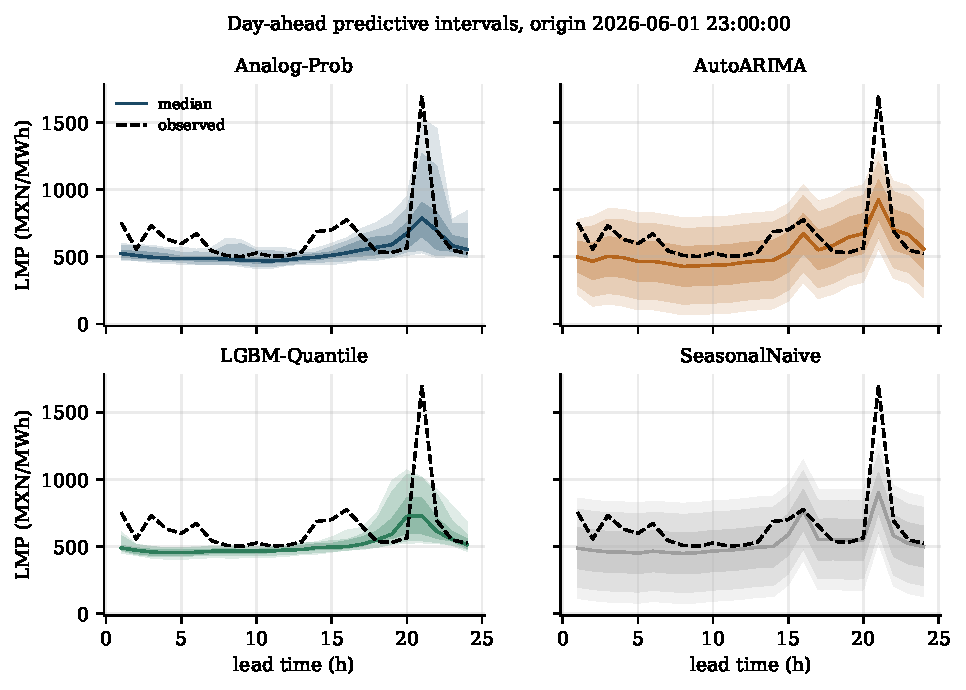
\includegraphics[width=\textwidth]{figs/fan.pdf}
\caption{Day-ahead predictive intervals (50\%, 80\% and 95\%) for one origin
of the test period. Dashed line: observed prices.}
\label{fig:fan}
\end{figure}

Figure~\ref{fig:crpstime} puts the two columns that decide whether a method
can be used in production side by side: the score, and the time it takes on a
logarithmic scale. The proposed method sits at the left end of the first and
near the left end of the second, three orders of magnitude away from
AutoARIMA.

\begin{figure}[htbp]
\centering
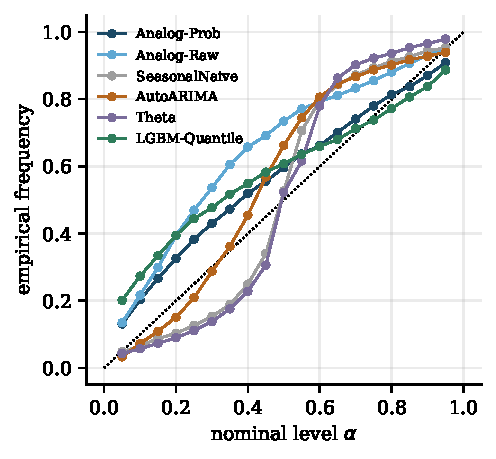
\includegraphics[width=0.55\textwidth]{figs/reliability.pdf}
\caption{Reliability diagram over the whole test period.}
\label{fig:reliability}
\end{figure}

\begin{figure}[htbp]
\centering
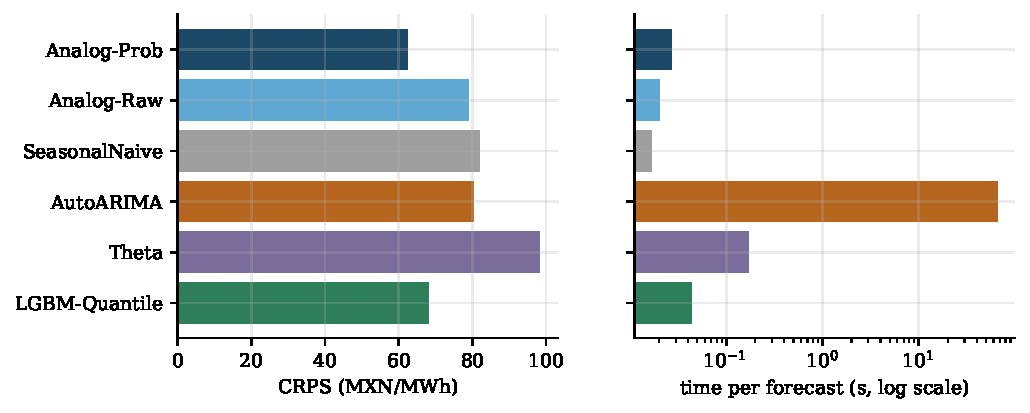
\includegraphics[width=\textwidth]{figs/crps_time.pdf}
\caption{Average CRPS (left) and computing time per forecast on a logarithmic
scale (right).}
\label{fig:crpstime}
\end{figure}

Table~\ref{tab:tail} looks only at the expensive side of the distribution,
which is the side that costs money to a buyer who hedges. The proposed method
has the lowest loss at the $0.95$ quantile, \APPINNINETYFIVE{} against
43 for the next best, even though its $95\%$ quantile is exceeded more
often than it should be: 9.1\% of the observations lie above it instead
of 5\%, and \APCOVNINETYFIVE{}\% of them fall inside the central $95\%$
interval. In other words, its upper quantile is in the right place more often
than the wider quantiles of the benchmarks, but it is still not high enough.
The gradient boosting, which is the sharpest of all, is also the one whose
interval is violated most often.

\begin{table}[htbp]
\centering
\caption{Upper-tail behaviour. Pinball loss at $\alpha=0.95$ and RMSE in
MXN/MWh; observed frequency below the 95\% quantile and exceedances of the
central 95\% interval in percent.}
\label{tab:tail}
\small
\begin{tabular}{lcccc}
\toprule
Method & Pinball$_{0.95}$ & $\hat a^{(0.95)}$ (\%) & Outside 95\% (\%) & RMSE \\
\midrule
Analog-Prob (this work) & \textbf{39.33} & 90.9 & 22.2 & 234.3 \\
Analog ensemble, $b_i=1$ (ablation) & 62.80 & 95.0 & 18.5 & 283.4 \\
Seasonal na\"ive & 51.35 & 95.3 & 9.6 & 285.3 \\
Dynamic optimized Theta & 43.11 & 97.9 & 6.4 & 274.5 \\
AutoARIMA$(p,d,q)(P,D,Q)_{24}$ & 53.62 & 94.0 & 9.3 & 266.7 \\
LightGBM quantile regression & 47.50 & 88.7 & 31.4 & 246.7 \\

\bottomrule
\end{tabular}
\end{table}

\subsection{Where the skill comes from}
\label{sec:ablation}

Table~\ref{tab:ablation} compares the three members of the family
\eqref{eq:family} on the same origins, together with the similarity-weighted
variant and with the output clipping disabled.

\begin{table}[htbp]
\centering
\caption{The member map decides the skill. All rows use the same analogs, the
same ensemble logic and the same evaluation; they differ only in the slope
$b_i$, in the weights, or in the clipping.}
\label{tab:ablation}
\small
\begin{tabular}{lcccccc}
\toprule
Member map & CRPS & $\Delta$ & Sharp. 95\% & Cov. 95\% & Pinball$_{0.95}$ & MAE \\
\midrule
$b_i=1$ (analog ensemble) & 79.0 & 0.257 & 806 & 0.815 & 62.80 & 197.2 \\
$b_i=\sigma_Y/\sigma_{X_i}$ (pattern rescaling) & 61.0 & 0.197 & 619 & 0.841 & 37.22 & 153.4 \\
$b_i=\rho_i\sigma_Y/\sigma_{X_i}$ (this work) & 62.3 & 0.216 & 515 & 0.778 & 39.33 & 156.2 \\
\quad with similarity weights & 62.1 & 0.212 & 572 & 0.808 & 38.23 & 156.1 \\
\quad without output clipping & 62.5 & 0.216 & 534 & 0.778 & 40.24 & 156.2 \\

\bottomrule
\end{tabular}
\end{table}

Two things are clear and one is uncomfortable. The first is that the
regression matters: the raw analog ensemble scores \ABANENCRPS{}, some
\ABOLSGAINANEN\% worse than the least-squares version, with the same analogs
and the same horizon. The analog search finds episodes of the right shape; it
is the pairwise map that brings each of them to the level of the present, and
without it the ensemble is both wider and worse.

The second is that the similarity weights change nothing, which is what one
should expect: the retained analogs all correlate strongly with the present,
so their weights are nearly equal. The output clip binds on \CLIPRATE\% of the
member-hours and changes the scores in the third digit.

The uncomfortable one is that the \emph{un-shrunk} rescaling does better than
least squares on this node. Its CRPS is \ABDUDCRPS{} against \ABOLSCRPS{}, its
deviation from nominal coverage \ABDUDREL{} against \ABOLSREL{}, its $95\%$
coverage \ABDUDCOV\% against \ABOLSCOV\%, and its loss at the $0.95$ quantile
\ABDUDPIN{} against \ABOLSPIN{}. The reason is the one that runs through this
whole section: the shrinkage factor $\rho_i<1$ pulls every member towards the
mean level of the present, which makes an ensemble that is already too narrow
narrower still. Least squares is the right answer to the question ``what is
the best point estimate of the present given this analog'' and the wrong answer
to the question ``how much can the future differ from it''.

We report this as an observation on one node and one test period, not as a
tuned choice: the configuration in Table~\ref{tab:main} was fixed before the
backtest and we have not changed it after seeing these numbers. Whether the
un-shrunk map dominates in general is a question for the multi-node study we
leave for future work.

\subsection{The ensemble is sharp but too narrow}
\label{sec:cal}

The under-coverage reported above is a property of the construction, not an
accident of this node: every member comes from an episode selected for
resembling the present, so the members resemble one another and the spread
between them understates the spread of what can actually happen. It can be
corrected without touching the method. Let $m_\tau$ be the median of the
ensemble at lead time $\tau$ and $s_\tau$ half the distance between its 10th
and 90th percentiles. Once an origin has been observed, the standardized error
$z_\tau=(y_\tau-m_\tau)/s_\tau$ is known. Using the pooled standardized errors
of the last $W$ observed origins, the recalibrated quantiles are
\begin{equation}
\hat Q^{\,c}_\tau(\alpha)\;=\;m_\tau+s_\tau\,\hat z(\alpha),
\label{eq:calib}
\end{equation}
where $\hat z(\alpha)$ is the empirical quantile of that pool. Nothing after
the origin is used, so the rule can be run in production. We take $W=20$
origins, which leaves \NCAL{} origins for evaluation.

Table~\ref{tab:calibration} reports the effect. Coverage at the $95\%$ level
rises from \CALCOVRAW\% to \CALCOV\%, and the deviation from nominal coverage
falls, at the price of intervals that widen from \CALSHARPRAW{} to
\CALSHARP{} MXN/MWh. The continuous ranked probability score barely moves
(\CALCRPSRAW{} against \CALCRPS{}), and the interval score deteriorates, from
\CALWINKRAW{} to \CALWINK{}. The reading we take from this is the honest one:
the narrowness of the ensemble is not a defect of the score, it is a defect of
the coverage. A user who needs intervals with the coverage they announce
should recalibrate and pay for it in width; a user who ranks forecasts by a
proper score should not.

\begin{table}[htbp]
\centering
\caption{Recalibration of the ensemble with the errors of past origins,
equation~\eqref{eq:calib}, on \NCAL{} origins. Scores in MXN/MWh.}
\label{tab:calibration}
\small
\begin{tabular}{lccccccc}
\toprule
& CRPS & $\Delta$ & Sharp. 95\% & Cov. 80\% & Cov. 95\% & Winkler & Pinball$_{0.95}$ \\
\midrule
Ensemble quantiles (as proposed) & 70.2 & 0.213 & 565 & 0.668 & 0.778 & 1\,271 & 46.01 \\
Recalibrated on past origins & 69.7 & 0.203 & 1\,059 & 0.791 & 0.894 & 1\,435 & 48.99 \\

\bottomrule
\end{tabular}
\end{table}

\subsection{Sensitivity to the parameters}
\label{sec:sens}

Table~\ref{tab:sensitivity} varies the present window $v_1$, the number of
analogs $k$ and the separation $\delta$ over a grid fixed in advance, on a
subsample of the origins. The grid was never used to choose the configuration
reported in Table~\ref{tab:main}.

\begin{table}[htbp]
\centering
\caption{Sensitivity of the probabilistic analog to its three parameters,
measured on \NSENS{} origins of the test period. CRPS in MXN/MWh.}
\label{tab:sensitivity}
\small
\begin{tabular}{ccccccc}
\toprule
$v_1$ (h) & $k$ & $\delta$ & CRPS & $\Delta$ & Cov. 95\% & Time (s) \\
\midrule
24 & 10 & 0.5 & 65.8 & 0.270 & 0.685 & 0.00 \\
24 & 10 & 1.0 & 66.4 & 0.271 & 0.683 & 0.00 \\
24 & 20 & 0.5 & 63.7 & 0.263 & 0.737 & 0.00 \\
24 & 20 & 1.0 & 63.6 & 0.264 & 0.737 & 0.00 \\
24 & 40 & 0.5 & 60.3 & 0.252 & 0.761 & 0.00 \\
24 & 40 & 1.0 & 60.1 & 0.252 & 0.767 & 0.00 \\
24 & 100 & 0.5 & 60.1 & 0.250 & 0.797 & 0.01 \\
24 & 100 & 1.0 & 59.4 & 0.246 & 0.799 & 0.01 \\
48 & 10 & 0.5 & 55.9 & 0.243 & 0.717 & 0.01 \\
48 & 10 & 1.0 & 54.9 & 0.237 & 0.721 & 0.01 \\
48 & 20 & 0.5 & 53.2 & 0.234 & 0.767 & 0.01 \\
48 & 20 & 1.0 & 53.3 & 0.235 & 0.761 & 0.01 \\
48 & 40 & 0.5 & 52.8 & 0.244 & 0.793 & 0.01 \\
48 & 40 & 1.0 & 52.2 & 0.239 & 0.797 & 0.01 \\
48 & 100 & 0.5 & 52.7 & 0.237 & 0.814 & 0.02 \\
48 & 100 & 1.0 & 52.9 & 0.235 & 0.826 & 0.02 \\
168 & 10 & 0.5 & 52.9 & 0.250 & 0.619 & 0.01 \\
168 & 10 & 1.0 & 53.3 & 0.250 & 0.621 & 0.01 \\
168 & 20 & 0.5 & \textbf{50.7} & 0.243 & 0.708 & 0.01 \\
168 & 20 & 1.0 & 50.9 & 0.243 & 0.710 & 0.02 \\
168 & 40 & 0.5 & 50.8 & 0.240 & 0.754 & 0.02 \\
168 & 40 & 1.0 & 51.0 & 0.238 & 0.746 & 0.02 \\
168 & 100 & 0.5 & 53.7 & 0.248 & 0.751 & 0.05 \\
168 & 100 & 1.0 & 52.9 & 0.244 & 0.757 & 0.25 \\

\bottomrule
\end{tabular}
\end{table}

The scores in Table~\ref{tab:sensitivity} are computed on a subsample and are
therefore not comparable with Table~\ref{tab:main}; what matters is their
ordering. Three regularities appear.

A longer present window helps, and by more than anything else in the grid: the
score improves monotonically from a one-day window to a two-day window and
again to a one-week window. A larger ensemble helps too, but with diminishing
and eventually negative returns, the best configuration being
$v_1=\SENSBESTV{}$, $k=\SENSBESTK{}$ and $\delta=\SENSBESTTOL{}$ at
\SENSBESTCRPS{}, against \SENSAPRIORI{} for the configuration we fixed in
advance — a gap of \SENSGAP\%. Our a priori choice was thus reasonable but not
optimal, which is the price of not tuning on the test period.

The separation rule is nearly inert. Changing $\delta$ from $0.5$ to $1$
barely moves any score, and the full $k$ analogs are retrieved in every
combination but one, the most demanding (a one-week window with a hundred
analogs and the strictest separation), where an average of $78$ analogs is
found. In this series $\delta$ decides \emph{which} analogs enter, not
\emph{how many}.

Finally, the cost is flat: between \SENSTMIN{} and \SENSTMAX{} seconds across
the whole grid. Neither $k$ nor $\delta$ moves it, and the window length moves
it only slightly, which confirms that the method pays for the search over
candidate windows and not for the regressions.

\section{Discussion}
\label{sec:discussion}

The result we consider most useful for operation is not the ranking but the
combination of the ranking with the cost column. A method that produces a full
predictive distribution in hundredths of a second can be run for every node of
a portfolio, every hour, on ordinary hardware, and can be re-run when new
information arrives. That was already the argument for the point version of
the analog method \citep{LezamaLope2023}, and it survives the move to
probabilistic forecasting because the extra cost of the probabilistic version
is $k$ univariate regressions, which is nothing next to the analog search that
both versions share.

The limits of the method should be stated plainly.

\textit{Resolution of the tails.} The predictive distribution has at most $k$
atoms per lead time, so quantiles outside $[1/(k+1),\,k/(k+1)]$ are not
estimated but interpolated by \eqref{eq:quantile}. With $k=\KANALOGS{}$ the
levels reported here are supported and the 99th percentile is not; a larger
ensemble, or a smoothing of it, would be required for statements about the far
tail.

\textit{Clipping.} The upper clip at the historical maximum means the method
cannot, by construction, forecast a price above any ever observed. For a
market with administrative price caps this is defensible, but it is an
assumption, not a result, and it makes the method conservative exactly in the
regime where prices are most extreme. It binds on \CLIPRATE\% of the
member-hours here, and Table~\ref{tab:ablation} shows what happens without it;
a method meant to warn about records should not carry it.

\textit{Selection and estimation share a statistic.} The similarity $\rho_i$
both admits an analog and sets its slope, so the fitted slopes are biased by
the selection. Splitting the present window — selecting on one half and
fitting on the other — is the natural check and is left for future work.

\textit{Members are not independent, and the ensemble is too narrow.} The
separation rule removes local duplicates, not statistical dependence: two
analogs a year apart may still be driven by the same seasonal pattern. Worse,
the members are selected precisely for resembling the present, so they resemble
one another, and the spread between them understates the spread of the future.
This is what the under-coverage of Section~\ref{sec:cal} measures. The
recalibration of \eqref{eq:calib} is a patch, not a cure: a construction that
produced calibrated members in the first place — for example by weighting
analogs by similarity in a way that admits dissimilar ones, or by adding the
residual dispersion of each pairwise fit to its member — would be preferable,
and we have not found one that keeps the score.

\textit{One node, one market, one season.} The evidence here is a single node
over six months. The relative ordering of the methods on another node, or in a
year with a different hydrological or fuel-price regime, has not been
established. We report the experiment as a reproducible starting point, not as
a general claim.

\textit{No exogenous information.} The method uses only the price history.
Load, temperature, fuel prices and scheduled outages are known to matter for
prices \citep{Weron2014,Uniejewski2019}, and a version of the analog search
that measures similarity on several variables at once is the natural next
step.

\textit{The path claim is not measured here.} Each member is a complete
trajectory, so the ensemble does carry the dependence between hours, which
methods that return marginal quantiles hour by hour do not. We have not
evaluated that dependence with a multivariate score such as the energy or the
variogram score, and therefore we do not claim the advantage, only the
property.

\textit{The horizon is bounded by the window.} The construction requires
$v_2\le v_1$, so the present window fixes the longest horizon the method can
produce in one shot. Longer horizons require chaining, which is what the point
version of the method does, and the effect of chaining on the coherence of the
trajectories has not been studied.

\section{Conclusions}
\label{sec:conclusions}

Making the analog method probabilistic does not require a new model. It
requires refusing to pool the analogs: fitting one regression per analog and
letting each of them speak produces an ensemble whose empirical quantiles
score better, on the day-ahead prices of the node studied here, than those of
standard statistical benchmarks and of a quantile gradient boosting, on every
score we measured and by a statistically significant margin, at a fraction of
the cost. The ablation shows that the regression step is essential rather than
cosmetic: without it, the same analogs score \CRPSGAINRAW\% worse. What the
method does not deliver out of the box is coverage — its intervals are too
narrow, and a user who needs the announced coverage must recalibrate them and
accept wider intervals. What is reported here is the analog stage made
probabilistic; the moving-average correction of \citet{LezamaLope2023} operates
on residuals and can be applied member by member, which would leave the
ensemble intact, and that composition is the first continuation we intend to
test. The others are a similarity measure over several variables, an ensemble
large enough to support statements about the far tail, and an evaluation of
the joint distribution across hours, which is what a buyer optimizing a
day-ahead purchase actually uses \citep{Rockafellar2000}.

\section*{Figure Legends}

\noindent\textbf{Figure 1.} Day-ahead predictive intervals (50\%, 80\% and
95\%) for one origin of the test period. The dashed line shows the observed
prices.

\noindent\textbf{Figure 2.} Reliability diagram over the whole test period.
The diagonal corresponds to a perfectly calibrated forecast.

\noindent\textbf{Figure 3.} Average continuous ranked probability score (left)
and computing time per forecast on a logarithmic scale (right).

\bibliographystyle{apacite}
\bibliography{references}

\end{document}
